%
% 6.S077 problem set solutions template
%
\documentclass[12pt,twoside]{article}
\usepackage{bbm}

\newcommand{\name}{}

\usepackage{amssymb}
\usepackage{amsmath}
\usepackage{graphicx}
\usepackage{latexsym}
\usepackage{times,url}
\usepackage{cprotect}
\usepackage{listings}
\usepackage{graphicx}
\usepackage[table]{xcolor}
\usepackage[letterpaper]{geometry}
\usepackage{tikz-qtree}
\usepackage{enumerate}

\newcommand{\profs}{Mauricio Karchmer, Aleksander Madry, Bruce Tidor}
\newcommand{\subj}{6.046}
\newcommand{\ttt}[1]{{\tt\small #1}}

\definecolor{dkgreen}{rgb}{0,0.6,0}
\definecolor{gray}{rgb}{0.5,0.5,0.5}
\definecolor{mauve}{rgb}{0.58,0,0.82}

\lstset{
  language=Python,
  aboveskip=1pc,
  belowskip=1pc,
  basicstyle={\footnotesize\ttfamily},
  numbers=left,
  showstringspaces=false,
  numberstyle=\tiny\color{gray},
  keywordstyle=\color{blue},
  commentstyle=\color{dkgreen},
  stringstyle=\color{mauve},
}

\tikzset{
  % every node/.style={minimum width=2em,draw,circle},
  % level 1/.style={sibling distance=2cm},
  level distance=1cm,
  edge from parent/.style=
  {draw,edge from parent path={(\tikzparentnode) -- (\tikzchildnode)}},
}

\newif\ifHideSolutions
\newcommand{\solution}[1]{\color{dkgreen}\textbf{Solution: }#1\color{black}}
\newcommand{\rubric}[1]{\color{dkgreen}{\bf Rubric:} #1\color{black}}

% \HideSolutionsfalse
% \ifHideSolutions
%   \renewcommand{\solution}[1]{}
%   \renewcommand{\rubric}[1]{}
% \fi

\newlength{\toppush}
\setlength{\toppush}{2\headheight}
\addtolength{\toppush}{\headsep}

\newcommand{\htitle}[2]{\noindent\vspace*{-\toppush}\newline\parbox{6.5in}
{\textit{Design and Analysis of Algorithms}\hfill\name\newline
Massachusetts Institute of Technology \hfill #2\newline
\profs\hfill #1 \vspace*{-.5ex}\newline
\mbox{}\hrulefill\mbox{}}\vspace*{1ex}\mbox{}\newline
\begin{center}{\Large\bf #1}\end{center}}

\newcommand{\handout}[2]{\thispagestyle{empty}
 \markboth{#1}{#1}
 \pagestyle{myheadings}\htitle{#1}{#2}}

\newcommand{\lecture}[3]{\thispagestyle{empty}
 \markboth{Lecture #1: #2}{Lecture #1: #2}
 \pagestyle{myheadings}\htitle{Lecture #1: #2}{#3}}

\newcommand{\htitlewithouttitle}[2]{\noindent\vspace*{-\toppush}\newline\parbox{6.5in}
{\textit{Design and Analysis of Algorithms}\hfill#2\newline
Massachusetts Institute of Technology \hfill 6.046\newline
\profs\hfill Handout #1\vspace*{-.5ex}\newline
\mbox{}\hrulefill\mbox{}}\vspace*{1ex}\mbox{}\newline}

\newcommand{\handoutwithouttitle}[2]{\thispagestyle{empty}
 \markboth{Handout \protect\ref{#1}}{Handout \protect\ref{#1}}
 \pagestyle{myheadings}\htitlewithouttitle{\protect\ref{#1}}{#2}}

\newcommand{\exam}[2]{% parameters: exam name, date
 \thispagestyle{empty}
 \markboth{\hspace{1cm}\subj\ #1\hspace{1in}Name\hrulefill\ \ }%
          {\subj\ #1\hspace{1in}Name\hrulefill\ \ }
 \pagestyle{myheadings}\examtitle{#1}{#2}
 \renewcommand{\theproblem}{Problem \arabic{problemnum}}
}
\newcommand{\examsolutions}[3]{% parameters: handout, exam name, date
 \thispagestyle{empty}
 \markboth{Handout \protect\ref{#1}: #2}{Handout \protect\ref{#1}: #2}
% \pagestyle{myheadings}\htitle{\protect\ref{#1}}{#2}{#3}
 \pagestyle{myheadings}\examsolutionstitle{\protect\ref{#1}} {#2}{#3}
 \renewcommand{\theproblem}{Problem \arabic{problemnum}}
}
\newcommand{\examsolutionstitle}[3]{\noindent\vspace*{-\toppush}\newline\parbox{6.5in}
{\textit{Design and Analysis of Algorithms}\hfill#3\newline
Massachusetts Institute of Technology \hfill 6.046\newline
%Singapore-MIT Alliance \hfill SMA5503\newline
\profs\hfill Handout #1\vspace*{-.5ex}\newline
\mbox{}\hrulefill\mbox{}}\vspace*{1ex}\mbox{}\newline
\begin{center}{\Large\bf #2}\end{center}}

\newcommand{\takehomeexam}[2]{% parameters: exam name, date
 \thispagestyle{empty}
 \markboth{\subj\ #1\hfill}{\subj\ #1\hfill}
 \pagestyle{myheadings}\examtitle{#1}{#2}
 \renewcommand{\theproblem}{Problem \arabic{problemnum}}
}

\makeatletter
\newcommand{\exambooklet}[2]{% parameters: exam name, date
 \thispagestyle{empty}
 \markboth{\subj\ #1}{\subj\ #1}
 \pagestyle{myheadings}\examtitle{#1}{#2}
 \renewcommand{\theproblem}{Problem \arabic{problemnum}}
 \renewcommand{\problem}{\newpage
 \item \let\@currentlabel=\theproblem
 \markboth{\subj\ #1, \theproblem}{\subj\ #1, \theproblem}}
}
\makeatother


\newcommand{\examtitle}[2]{\noindent\vspace*{-\toppush}\newline\parbox{6.5in}
{\textit{Design and Analysis of Algorithms}\hfill#2\newline
Massachusetts Institute of Technology \hfill 6.046 Spring 2019\newline
%Singapore-MIT Alliance \hfill SMA5503\newline
\profs\hfill #1\vspace*{-.5ex}\newline
\mbox{}\hrulefill\mbox{}}\vspace*{1ex}\mbox{}\newline
\begin{center}{\Large\bf #1}\end{center}}

\newcommand{\grader}[1]{\hspace{1cm}\textsf{\textbf{#1}}\hspace{1cm}}

\newcommand{\points}[1]{[#1 points]\ }
\newcommand{\parts}[1]
{
  \ifnum#1=1
  (1 part)
  \else
  (#1 parts)
  \fi
  \ 
}

\newcommand{\bparts}{\begin{problemparts}}
\newcommand{\eparts}{\end{problemparts}}
\newcommand{\ppart}{\problempart}

%\newcommand{\lg} {lg\ }

\setlength{\oddsidemargin}{0pt}
\setlength{\evensidemargin}{0pt}
\setlength{\textwidth}{6.5in}
\setlength{\topmargin}{0in}
\setlength{\textheight}{8.5in}


\newcommand{\Spawn}{{\bf spawn} }
\newcommand{\Sync}{{\bf sync}}

\newcommand{\cif}[1]{\mbox{if $#1$}}
\newcommand{\cwhen}[1]{\mbox{when $#1$}}

\newcounter{problemnum}
\newcommand{\theproblem}{Problem \theproblemsetnum-\arabic{problemnum}}
\newenvironment{problems}{
        \begin{list}{{\bf \theproblem. \hspace*{0.5em}}}
        {\setlength{\leftmargin}{0em}
         \setlength{\rightmargin}{0em}
         \setlength{\labelwidth}{0em}
         \setlength{\labelsep}{0em}
         \usecounter{problemnum}}}{\end{list}}
\makeatletter
\newcommand{\problem}[1][{}]{\item \let\@currentlabel=\theproblem \textbf{#1}}
\makeatother

\newcounter{problempartnum}[problemnum]
\newenvironment{problemparts}{
        \begin{list}{{\bf (\alph{problempartnum})}}
        {\setlength{\leftmargin}{2.5em}
         \setlength{\rightmargin}{2.5em}
         \setlength{\labelsep}{0.5em}}}{\end{list}}
\newcommand{\problempart}{\addtocounter{problempartnum}{1}\item}

\newenvironment{truefalseproblemparts}{
        \begin{list}{{\bf (\alph{problempartnum})\ \ \ T\ \ F\hfil}}
        {\setlength{\leftmargin}{4.5em}
         \setlength{\rightmargin}{2.5em}
         \setlength{\labelsep}{0.5em}
         \setlength{\labelwidth}{4.5em}}}{\end{list}}

\newcounter{exercisenum}
\newcommand{\theexercise}{Exercise \theproblemsetnum-\arabic{exercisenum}}
\newenvironment{exercises}{
        \begin{list}{{\bf \theexercise. \hspace*{0.5em}}}
        {\setlength{\leftmargin}{0em}
         \setlength{\rightmargin}{0em}
         \setlength{\labelwidth}{0em}
         \setlength{\labelsep}{0em}
        \usecounter{exercisenum}}}{\end{list}}
\makeatletter
\newcommand{\exercise}{\item \let\@currentlabel=\theexercise}
\makeatother

\newcounter{exercisepartnum}[exercisenum]
%\newcommand{\problem}[1]{\medskip\mbox{}\newline\noindent{\bf Problem #1.}\hspace*{1em}}
%\newcommand{\exercise}[1]{\medskip\mbox{}\newline\noindent{\bf Exercise #1.}\hspace*{1em}}

\newenvironment{exerciseparts}{
        \begin{list}{{\bf (\alph{exercisepartnum})}}
        {\setlength{\leftmargin}{2.5em}
         \setlength{\rightmargin}{2.5em}
         \setlength{\labelsep}{0.5em}}}{\end{list}}
\newcommand{\exercisepart}{\addtocounter{exercisepartnum}{1}\item}


% Macros to make captions print with small type and 'Figure xx' in bold.
\makeatletter
\def\fnum@figure{{\bf Figure \thefigure}}
\def\fnum@table{{\bf Table \thetable}}
\let\@mycaption\caption
%\long\def\@mycaption#1[#2]#3{\addcontentsline{\csname
%  ext@#1\endcsname}{#1}{\protect\numberline{\csname 
%  the#1\endcsname}{\ignorespaces #2}}\par
%  \begingroup
%    \@parboxrestore
%    \small
%    \@makecaption{\csname fnum@#1\endcsname}{\ignorespaces #3}\par
%  \endgroup}
%\def\mycaption{\refstepcounter\@captype \@dblarg{\@mycaption\@captype}}
%\makeatother
\let\mycaption\caption
%\newcommand{\figcaption}[1]{\mycaption[]{#1}}

\newcounter{totalcaptions}
\newcounter{totalart}

\newcommand{\figcaption}[1]{\addtocounter{totalcaptions}{1}\caption[]{#1}}

% \psfigures determines what to do for figures:
%       0 means just leave vertical space
%       1 means put a vertical rule and the figure name
%       2 means insert the PostScript version of the figure
%       3 means put the figure name flush left or right
\newcommand{\psfigures}{0}
\newcommand{\spacefigures}{\renewcommand{\psfigures}{0}}
\newcommand{\rulefigures}{\renewcommand{\psfigures}{1}}
\newcommand{\macfigures}{\renewcommand{\psfigures}{2}}
\newcommand{\namefigures}{\renewcommand{\psfigures}{3}}

\newcommand{\figpart}[1]{{\bf (#1)}\nolinebreak[2]\relax}
\newcommand{\figparts}[2]{{\bf (#1)--(#2)}\nolinebreak[2]\relax}


\macfigures     % STATE

% When calling \figspace, make sure to leave a blank line afterward!!
% \widefigspace is for figures that are more than 28pc wide.
\newlength{\halffigspace} \newlength{\wholefigspace}
\newlength{\figruleheight} \newlength{\figgap}
\newcommand{\setfiglengths}{\ifnum\psfigures=1\setlength{\figruleheight}{\hruleheight}\setlength{\figgap}{1em}\else\setlength{\figruleheight}{0pt}\setlength{\figgap}{0em}\fi}
\newcommand{\figspace}[2]{\ifnum\psfigures=0\leavefigspace{#1}\else%
\setfiglengths%
\setlength{\wholefigspace}{#1}\setlength{\halffigspace}{.5\wholefigspace}%
\rule[-\halffigspace]{\figruleheight}{\wholefigspace}\hspace{\figgap}#2\fi}
\newlength{\widefigspacewidth}
% Make \widefigspace put the figure flush right on the text page.
\newcommand{\widefigspace}[2]{
\ifnum\psfigures=0\leavefigspace{#1}\else%
\setfiglengths%
\setlength{\widefigspacewidth}{28pc}%
\addtolength{\widefigspacewidth}{-\figruleheight}%
\setlength{\wholefigspace}{#1}\setlength{\halffigspace}{.5\wholefigspace}%
\makebox[\widefigspacewidth][r]{#2\hspace{\figgap}}\rule[-\halffigspace]{\figruleheight}{\wholefigspace}\fi}
\newcommand{\leavefigspace}[1]{\setlength{\wholefigspace}{#1}\setlength{\halffigspace}{.5\wholefigspace}\rule[-\halffigspace]{0em}{\wholefigspace}}

% Commands for including figures with macpsfig.
% To use these commands, documentstyle ``macpsfig'' must be specified.
\newlength{\macfigfill}
\makeatother
\newlength{\bbx}
\newlength{\bby}
\newcommand{\macfigure}[5]{\addtocounter{totalart}{1}
\ifnum\psfigures=2%
\setlength{\bbx}{#2}\addtolength{\bbx}{#4}%
\setlength{\bby}{#3}\addtolength{\bby}{#5}%
\begin{flushleft}
\ifdim#4>28pc\setlength{\macfigfill}{#4}\addtolength{\macfigfill}{-28pc}\hspace*{-\macfigfill}\fi%
\mbox{\psfig{figure=./#1.ps,%
bbllx=#2,bblly=#3,bburx=\bbx,bbury=\bby}}
\end{flushleft}%
\else\ifdim#4>28pc\widefigspace{#5}{#1}\else\figspace{#5}{#1}\fi\fi}
\makeatletter

\newlength{\savearraycolsep}
\newcommand{\narrowarray}[1]{\setlength{\savearraycolsep}{\arraycolsep}\setlength{\arraycolsep}{#1\arraycolsep}}
\newcommand{\normalarray}{\setlength{\arraycolsep}{\savearraycolsep}}

\newcommand{\hint}{{\em Hint:\ }}

% Macros from /th/u/clr/mac.tex

\newcommand{\set}[1]{\left\{ #1 \right\}}
\newcommand{\abs}[1]{\left| #1\right|}
\newcommand{\card}[1]{\left| #1\right|}
\newcommand{\floor}[1]{\left\lfloor #1 \right\rfloor}
\newcommand{\ceil}[1]{\left\lceil #1 \right\rceil}
\newcommand{\ang}[1]{\ifmmode{\left\langle #1 \right\rangle}
   \else{$\left\langle${#1}$\right\rangle$}\fi}
        % the \if allows use outside mathmode,
        % but will swallow following space there!
\newcommand{\paren}[1]{\left( #1 \right)}
\newcommand{\bracket}[1]{\left[ #1 \right]}
\newcommand{\prob}[1]{\Pr\left\{ #1 \right\}}
\newcommand{\Var}{\mathop{\rm Var}\nolimits}
\newcommand{\expect}[1]{{\rm E}\left[ #1 \right]}
\newcommand{\expectsq}[1]{{\rm E}^2\left[ #1 \right]}
\newcommand{\variance}[1]{{\rm Var}\left[ #1 \right]}
\renewcommand{\choose}[2]{{{#1}\atopwithdelims(){#2}}}
\def\pmod#1{\allowbreak\mkern12mu({\rm mod}\,\,#1)}
\newcommand{\matx}[2]{\left(\begin{array}{*{#1}{c}}#2\end{array}\right)}
\newcommand{\Adj}{\mathop{\rm Adj}\nolimits}

\newtheorem{theorem}{Theorem}
\newtheorem{lemma}[theorem]{Lemma}
\newtheorem{corollary}[theorem]{Corollary}
\newtheorem{xample}{Example}
\newtheorem{definition}{Definition}
\newenvironment{example}{\begin{xample}\rm}{\end{xample}}
\newcommand{\proof}{\noindent{\em Proof.}\hspace{1em}}
\def\squarebox#1{\hbox to #1{\hfill\vbox to #1{\vfill}}}
\newcommand{\qedbox}{\vbox{\hrule\hbox{\vrule\squarebox{.667em}\vrule}\hrule}}
\newcommand{\qed}{\nopagebreak\mbox{}\hfill\qedbox\smallskip}
\newcommand{\eqnref}[1]{(\protect\ref{#1})}

%%\newcommand{\twodots}{\mathinner{\ldotp\ldotp}}
\newcommand{\transpose}{^{\mbox{\scriptsize \sf T}}}
\newcommand{\amortized}[1]{\widehat{#1}}

\newcommand{\punt}[1]{}

%%% command for putting definitions into boldface
% New style for defined terms, as of 2/23/88, redefined by THC.
\newcommand{\defn}[1]{{\boldmath\textit{\textbf{#1}}}}
\newcommand{\defi}[1]{{\textit{\textbf{#1\/}}}}

\newcommand{\red}{\leq_{\rm P}}
\newcommand{\lang}[1]{%
\ifmmode\mathord{\mathcode`-="702D\rm#1\mathcode`\-="2200}\else{\rm#1}\fi}

%\newcommand{\ckt}[1]{\ifmmode\mathord{\mathcode`-="702D\sc #1\mathcode`\-="2200}\else$\mathord{\mathcode`-="702D\sc #1\mathcode`\-="2200}$\fi}
\newcommand{\ckt}[1]{\ifmmode \sc #1\else$\sc #1$\fi}

%% Margin notes - use \notesfalse to turn off notes.
\setlength{\marginparwidth}{0.6in}
\reversemarginpar
\newif\ifnotes
\notestrue
\newcommand{\longnote}[1]{
  \ifnotes
    {\medskip\noindent Note: \marginpar[\hfill$\Longrightarrow$]
      {$\Longleftarrow$}{#1}\medskip}
  \fi}
\newcommand{\note}[1]{
  \ifnotes
    {\marginpar{\tiny \raggedright{#1}}}
  \fi}


\newcommand{\reals}{\mathbbm{R}}
\newcommand{\integers}{\mathbbm{Z}}
\newcommand{\naturals}{\mathbbm{N}}
\newcommand{\rationals}{\mathbbm{Q}}
\newcommand{\complex}{\mathbbm{C}}

\newcommand{\oldreals}{{\bf R}}
\newcommand{\oldintegers}{{\bf Z}}
\newcommand{\oldnaturals}{{\bf N}}
\newcommand{\oldrationals}{{\bf Q}}
\newcommand{\oldcomplex}{{\bf C}}

\newcommand{\w}{\omega}                 %% for fft chapter

\newenvironment{closeitemize}{\begin{list}
{$\bullet$}
{\setlength{\itemsep}{-0.2\baselineskip}
\setlength{\topsep}{0.2\baselineskip}
\setlength{\parskip}{0pt}}}
{\end{list}}

% These are necessary within a {problems} environment in order to restore
% the default separation between bullets and items.
\newenvironment{normalitemize}{\setlength{\labelsep}{0.5em}\begin{itemize}}
                              {\end{itemize}}
\newenvironment{normalenumerate}{\setlength{\labelsep}{0.5em}\begin{enumerate}}
                                {\end{enumerate}}

%\def\eqref#1{Equation~(\ref{eq:#1})}
%\newcommand{\eqref}[1]{Equation (\ref{eq:#1})}
\newcommand{\eqreftwo}[2]{Equations (\ref{eq:#1}) and~(\ref{eq:#2})}
\newcommand{\ineqref}[1]{Inequality~(\ref{ineq:#1})}
\newcommand{\ineqreftwo}[2]{Inequalities (\ref{ineq:#1}) and~(\ref{ineq:#2})}

\newcommand{\figref}[1]{Figure~\ref{fig:#1}}
\newcommand{\figreftwo}[2]{Figures \ref{fig:#1} and~\ref{fig:#2}}

\newcommand{\liref}[1]{line~\ref{li:#1}}
\newcommand{\Liref}[1]{Line~\ref{li:#1}}
\newcommand{\lirefs}[2]{lines \ref{li:#1}--\ref{li:#2}}
\newcommand{\Lirefs}[2]{Lines \ref{li:#1}--\ref{li:#2}}
\newcommand{\lireftwo}[2]{lines \ref{li:#1} and~\ref{li:#2}}
\newcommand{\lirefthree}[3]{lines \ref{li:#1}, \ref{li:#2}, and~\ref{li:#3}}

\newcommand{\lemlabel}[1]{\label{lem:#1}}
\newcommand{\lemref}[1]{Lemma~\ref{lem:#1}} 

\newcommand{\exref}[1]{Exercise~\ref{ex:#1}}

\newcommand{\handref}[1]{Handout~\ref{#1}}

\newcommand{\defref}[1]{Definition~\ref{def:#1}}

% (1997.8.16: Victor Luchangco)
% Modified \hlabel to only get date and to use handouts counter for number.
%   New \handout and \handoutwithouttitle commands in newmac.tex use this.
%   The date is referenced by <label>-date.
%   (Retained old definition as \hlabelold.)
%   Defined \hforcelabel to use an argument instead of the handouts counter.

\newcounter{handouts}
\setcounter{handouts}{0}

\newcommand{\hlabel}[2]{%
\stepcounter{handouts}
{\edef\next{\write\@auxout{\string\newlabel{#1}{{\arabic{handouts}}{0}}}}\next}
\write\@auxout{\string\newlabel{#1-date}{{#2}{0}}}
}

\newcommand{\hforcelabel}[3]{%          Does not step handouts counter.
\write\@auxout{\string\newlabel{#1}{{#2}{0}}}
\write\@auxout{\string\newlabel{#1-date}{{#3}{0}}}}


% less ugly underscore
% --juang, 2008 oct 05
\renewcommand{\_}{\vrule height 0 pt depth 0.4 pt width 0.5 em \,}

\newcommand{\theproblemsetnum}{8}
\newcommand{\releasedate}{Tuesday, April 23}
\newcommand{\partaduedate}{Tuesday, May 7}
\allowdisplaybreaks

\title{6.S077 Problem Set \theproblemsetnum}

\begin{document}

\handout{Problem Set \theproblemsetnum}{\releasedate}
\textbf{All parts are due {\bf \partaduedate} at {\bf 2:30PM}}.

\setlength{\parindent}{0pt}
\medskip\hrulefill\medskip

{\bf Name:} Robert Durfee

\medskip

{\bf Collaborators:} None

\medskip\hrulefill

\begin{problems}

\problem  % Problem 1

\begin{problemparts}

\problempart  % Problem 1a

The definition of the $G$-statistic is,
$$ G = -2 \log \left(\frac{\sup_{\theta \in
\Theta_0}\mathcal{L}(\theta)}{\sup_{\theta \in \Theta}
\mathcal{L}(\theta)}\right) $$
Since we are testing the hypothesis,
$$ H : p = 1/2 $$
$$ K : p \neq 1/2 $$
We have the following,
$$ \Theta_0 = \{p\}, \quad \Theta = [0, 1] $$
Using this, the $G$-statistic simplifies to,
\begin{align*}
    G &= -2 \log \left(\frac{\mathcal{L}(p)}{\max_{\theta \in [0, 1]}
    \mathcal{L}(\theta)}\right) \\
    &= -2 \log \left(\frac{\mathbb{P}(x_1, \ldots, x_n \mid p)}{\max_{\theta
    \in [0, 1]} \mathbb{P}(x_1,\ldots,x_n \mid \theta)}\right)\\
    &= -2 \log \left(\frac{\prod_{i = 1}^n \mathbb{P}(x_i\mid
    p)}{\max_{\theta \in [0, 1]} \prod_{i = 1}^n \mathbb{P}(x_i\mid
    \theta)}\right)
\end{align*}
If we define the following empirical quantity,
$$ \bar{X}_n = \frac{1}{n} \sum_{i = 1}^n x_i $$
We can write the $G$-statistic as,
$$ G = -2 \log \left(\frac{p^{n \bar{X}_n} (1 - p)^{n(1 -
\bar{X}_n)}}{\max_{\theta \in [0, 1]} \theta^{n \bar{X}_n} (1 - \theta)^{n(1
- \bar{X}_n)}}\right) $$
We can maximize the denominator to get $\theta^*$,
\begin{align*}
    \theta^* &= \arg\max_{\theta \in [0, 1]} \theta^{n \bar{X}_n} (1 -
    \theta)^{n(1 - \bar{X}_n)} \\
    &= \arg\max_{\theta \in [0, 1]} n \bar{X}_n \log \theta + n(1 -
    \bar{X}_n) \log (1 - \theta) \\
\end{align*}
Taking the derivative of the expression with respect to $\theta$,
$$ \frac{\partial}{\partial \theta}(\cdot) = \frac{n \bar{X}_n}{\theta} -
\frac{n(1 - \bar{X}_n)}{1 - \theta} $$
Setting this equal to zero and solving for $\theta^*$,
\begin{align*}
    0 &= \frac{n \bar{X}_n}{\theta^*} - \frac{n(1 - \bar{X}_n)}{1 - \theta^*} \\
    \frac{n \bar{X}_n}{\theta^*} &= \frac{n(1 - \bar{X}_n)}{1 - \theta^*} \\
    (1 - \theta^*) \bar{X}_n &= \theta^* (1 - \bar{X}_n) \\
    \bar{X}_n - \theta^* \bar{X}_n &= \theta^* - \theta^* \bar{X}_n \\
    \theta^* &= \bar{X}_n
\end{align*}
Therefore, the $G$-statistic becomes,
\begin{align*}
    G &= -2 \log \left(\frac{p^{n \bar{X}_n} (1 - p)^{n(1 -
    \bar{X}_n)}}{\bar{X}_n^{n \bar{X}_n} (1 - \bar{X}_n)^{n(1 -
    \bar{X}_n)}}\right) \\
    &= -2 \left(n \bar{X}_n \log p + n(1 - \bar{X}_n) \log (1 - p) -
    n\bar{X}_n \log \bar{X}_n - n(1 - \bar{X}_n)\log(1 - \bar{X}_n)\right)
\end{align*}
Since $p = 1/2$, this reduces to,
$$ \boxed{G = 2n \left(1 + \bar{X}_n \log \bar{X}_n + (1 - \bar{X}_n)\log(1 -
\bar{X}_n)\right)} $$
To find the threshold value, consider the following probability,
$$ \mathbb{P}\left(G > g_\alpha\right) = \alpha $$
Substituting the $G$-statistic,
\begin{align*}
    \mathbb{P}\left(2 n \left(1 + \bar{X}_n \log \bar{X}_n + (1 -
    \bar{X}_n)\log(1 - \bar{X}_n)\right) > g_\alpha\right) &= \alpha \\
    \mathbb{P}\left(\bar{X}_n \log \bar{X}_n + (1 - \bar{X}_n)\log(1 -
    \bar{X}_n) > \frac{g_\alpha}{2n} - 1\right) &= \alpha
\end{align*}
If we use the definition of binary entropy,
$$ h(p) = - p \log p - (1 - p) \log (1 - p) $$
This $G$-statistic further reduces to,
$$ \mathbb{P}\left(h(\bar{X}_n) < 1 - \frac{g_\alpha}{2n}\right) = \alpha $$
Given that $n \bar{X}_n \sim \mathrm{Binomial}(n, p)$ and $n = 10, p = 1/2,
\alpha = 0.109375$, we note the following,
$$ \mathbb{P}(10 \cdot \bar{X}_{10} > 7) = \mathbb{P}(10 \cdot \bar{X}_{10} <
3) = \frac{0.109375}{2} $$
Therefore, the $G$-statistic becomes,
$$ \mathbb{P}\left(h(0.3) < 1 - \frac{g_\alpha}{20}\right) = 0.109375 $$
Solving for the threshold $g_\alpha$ yields,
$$ g_\alpha = 20(1 - h(0.3)) \approx \boxed{2.37418} $$

\problempart  % Problem 1b

The definition of the $Z$-statistic with known variance is,
$$ Z = \frac{\sum_{i = 1}^n (x_i - \mu_0)}{\sqrt{n \sigma_0^2}} $$
This is equivalent to,
$$ Z = \left(\frac{1}{n} \sum_{i = 1}^n x_i - \mu_0\right)
\sqrt{\frac{n}{\sigma_0^2}} $$
In this case, since $x_i \sim \mathrm{Bernoulli}(p)$, this reduces to,
$$ Z = \left(\frac{1}{n}\sum_{i = 1}^n x_i - p\right)\sqrt{\frac{n}{p(1 -
p)}} $$
If we define the same quantity as above,
$$ \bar{X}_n = \frac{1}{n} \sum_{i = 1}^n x_i $$
This then becomes,
$$ \boxed{Z = \left(\bar{X}_n - p\right)\sqrt{\frac{n}{p(1 - p)}}} $$
To compute the threshold, consider the following probability,
$$ \mathbb{P}(|Z| > z_\alpha) = \alpha $$
Substituting the $Z$-statistic,
$$ \mathbb{P}\left(\left|\left(\bar{X}_n - p\right)\sqrt{\frac{n}{p(1 -
p)}}\right| > z_\alpha\right) = \alpha $$
Given that $n \bar{X}_n \sim \mathrm{Binomial}(n, p)$ and $n = 10, p = 1/2,
\alpha = 0.109375$, we again note the following,
$$ \mathbb{P}(10 \cdot \bar{X}_{10} > 7) = \mathbb{P}(10 \cdot \bar{X}_{10} <
3) = \frac{0.109375}{2} $$
Therefore, the $Z$-statistic becomes,
$$ \mathbb{P}\left(\left|(0.7 - 1/2) \sqrt{\frac{10}{1/4}}\right| > z_\alpha
\right) = \alpha $$
Solving for $z_\alpha$ yields,
$$ z_\alpha = \left|(0.7 - 1/2) \sqrt{\frac{10}{1/4}}\right| \approx
\boxed{1.26491} $$

\problempart  % Problem 1c

First we consider the rejection region for the $G$-statistic,
$$ \left\{h(\bar{X}_n) \leq 1 - \frac{g_\alpha}{2n}\right\} $$
Let $t_1$ be some threshold such that
$$ h(t_1) = 1 - \frac{g_\alpha}{2n} $$
Due to the symmetry of the binary entropy function, the following will also
hold,
$$ h(1 - t_1) = 1 - \frac{g_\alpha}{2n} $$
Therefore, the set of all $\bar{X}_n$ that satisfy this rejection region are,
$$ \{\bar{X}_n \leq t_1\} \cup \{\bar{X}_n \geq 1 - t_1\} $$
Applying a simple transformation yields,
$$ \{\bar{X}_n - 1/2 \leq t_1 - 1/2\} \cup \{\bar{X}_n - 1/2 \geq 1/2 - t_1\}
$$
This can be rewritten as,
$$ \boxed{\{| \bar{X}_n - 1/2 | \geq 1/2 - t_1 \}} $$

Now we consider the rejection region for the $Z$-statistic,
$$ \left\{\left|(\bar{X}_n - 1/2) \sqrt{\frac{n}{1/4}}\right| \geq
z_\alpha\right\} $$
If we let $t_2 = z_\alpha$, after some rearranging,
$$ \boxed{\left\{\left|\bar{X}_n - 1/2 \right| \geq
t_2\sqrt{\frac{1/4}{n}}\right\}} $$

It is important to note that there exists a $t_1$ and $t_2$ such that both
rejection regions are equivalent. Therefore, neither test is better than the
other.

\end{problemparts}

\newpage

\problem  % Problem 2

\begin{problemparts}

\problempart  % Problem 2a

Consider the following hypothesis,
$$ H_0 : \pi = 1/2 $$
$$ H_1 : \pi \neq 1/2 $$
Since this is a $x_1 \sim \mathrm{Bernoulli}(\pi)$, we know the variance
under the null hypothesis. Thus, we use a $Z$-test. Consider the
$Z$-statistic,
\begin{align*}
    Z &= \frac{\sum_{i = 1}^n (x_i - \mu_0)}{\sqrt{n \sigma_0^2}} \\
    &= \frac{\sum_{i = 1}^{82} (b_i - 1/2)}{\sqrt{938223 \cdot (1/4)}} \\
    &= \frac{484382 - 938223/2}{\sqrt{938223/4}} \\
    &\approx 31.5305
\end{align*}
Using the standard normal approximation, the corresponding $p$-value is,
$$ \mathbb{P}(|Z| > 31.5305) \approx \boxed{3.3187 \cdot 10^{-218}} $$
Therefore, we have strong evidence to reject the null that $\pi = 1/2$

\problempart  % Problem 2b

Now consider the following hypothesis,
$$ H_0 : \pi = 0.515 $$
$$ H_1 : \pi \neq 0.515 $$
Consider the $Z$-statistic,
\begin{align*}
    Z &= \frac{\sum_{i = 1}^n (x_i - \mu_0)}{\sqrt{n \sigma_0^2}} \\
    &= \frac{\sum_{i = 1}^{82} (b_i - 0.515)}{\sqrt{938223 \cdot 0.515 \cdot
    (1 - 0.515)}} \\
    &= \frac{484382 - 938223 \cdot 0.515}{\sqrt{938223 \cdot 0.515 \cdot (1 -
    0.515)}} \\
    &\approx 2.47299
\end{align*}
Using the standard normal approximation, the corresponding $p$-value is,
$$ \mathbb{P}(|Z| > 2.47299) \approx \boxed{0.0134} $$
Therefore, it is not nearly as convincing to reject the null.

\problempart  % Problem 2c

Consider the empirical value of the variance under the null,
$$ \hat{\sigma}_0^2 = \frac{1}{n} \sum_{i = 1}^{82} (b_i - n_i \pi)^2 $$
This can be rewritten as,
$$ \hat{\sigma}_0^2\frac{1}{n}\left(\sum_{i = 1}^{82} b_i^2 - 2 \pi \sum_{i =
1}^{82} b_i n_i + \pi^2 \sum_{i = 1}^{82} n_i^2\right) $$
Substituting provided terms,
\begin{align*}
    \hat{\sigma}_0^2 &= \frac{1}{938223}\left(3082550890 - 2 \cdot 18/35
    \cdot 5975723599 + (18/35)^2 \cdot 11586072783\right) \\
    &\approx \boxed{0.522644}
\end{align*}

Now consider the expected variance under the null,
\begin{align*}
    \mathbb{E}[\sigma_0^2] &= \mathbb{E}\left[\frac{1}{n} \sum_{i = 1}^{82}
    (b_i - n_i \pi)^2\right] \\
    &= \frac{1}{n} \sum_{i = 1}^{82} \mathbb{E}[b_i^2] - 2 \pi n_i
    \mathbb{E}[b_i] + \pi^2 n_i^2
\end{align*}
Using the fact that $b_i \sim \mathrm{Binomial}(n_i, \pi)$, we know,
$$ \mathbb{E}[b_i] = n_i \pi,\ \mathbb{E}[b_i^2] = n_i \pi (1 - \pi) + \pi^2
n_i^2 $$
Substituting into the expectation,
\begin{align*}
    \mathbb{E}[\sigma_0^2] &= \frac{1}{n} \sum_{i = 1}^{82} n_i \pi (1 - \pi) \\
    &= \frac{\pi (1 - \pi)}{n} \sum_{i = 1}^{82} n_i \\
    &= \pi (1 - \pi) \\
    &= (18/35) (1 - 18/35) \\
    &\approx \boxed{0.24979}
\end{align*}

From this, we do not think that the variance was too low. In fact, the
variance is significantly higher than expected.

\end{problemparts}

\newpage

\problem  % Problem 3

Consider the following hypothesis,
$$ H_0 : \mu_L = \mu_R $$
$$ H_1 : \mu_L < \mu_R $$
If we let $\theta = \mu_L - \mu_R$, this is equivalent to,
$$ H_0 : \theta = 0 $$
$$ H_1 : \theta < 0 $$
We can construct the two sample $T$-statistic,
$$ T = \frac{\bar{X}_L - \bar{X}_R}{\sqrt{\hat{\sigma}_L^2/n_L +
\hat{\sigma}_R^2/n_R}} $$
The empirical variance for a set of Bernoulli random variables is
$$ \hat{\sigma}^2 = \frac{1}{n} \sum_{i = 1}^n (x_i - \bar{X})^2 = \bar{X} (1
- \bar{X}) $$
Therefore, from the data, we get the following proportions,
$$ \bar{X}_L = \frac{130866}{130866 + 139782} \approx 0.483528 $$
$$ \bar{X}_R = \frac{3083}{3083 + 3256} \approx 0.486354 $$
Using these, we can get the variances,
$$ \hat{\sigma}_L^2 = 0.483528 (1 - 0.483528) \approx 0.249729 $$
$$ \hat{\sigma}_R^2 = 0.486354 (1 - 0.486354) \approx 0.249813 $$
Substituting into the $T$-statistic,
\begin{align*}
    T &= \frac{0.483528 - 0.486354}{\sqrt{0.249729/270648 + 0.249813/6339}} \\
    &\approx -0.444989
\end{align*}
Calculating the $p$-value using the normal approximation,
$$ \mathbb{P}(T \leq -0.444989) \approx \boxed{0.326355} $$
Since the probability of this value occuring or a value more extreme is
roughly 33\%, I do not think this result is significant.

\newpage

\problem  % Problem 4

\begin{problemparts}

\problempart  % Problem 4a

Using the definition of $L$ given in the problem set,
$$ L = \sum_{i = 1}^n \log \frac{P(X_i)}{Q(X_i)} $$
In this sense, if the null is rejected what $L > t$, then when the null is
incorrect, we want the ratio to approach infinity. Therefore,
$$ P : X_i \sim \mathcal{N}(a_i, 1) $$
$$ Q : X_i \sim \mathcal{N}(0, 1) $$
Therefore, the likelihood ratio statistic is,
\begin{align*}
    L &= \sum_{i = 1}^n \log \frac{\exp\{-(x_i -
    a_i)^2/2\}}{\exp\{-x_i^2/2\}} \\
    &= \frac{1}{2}\sum_{i = 1}^n x_i^2 - (x_i - a_i)^2 \\
    &= \frac{1}{2}\sum_{i = 1}^n 2 x_i a_i - a_i^2
\end{align*}
The rejection rule would then become,
$$ \boxed{\frac{1}{2}\sum_{i = 1}^n 2 x_i a_i - a_i^2 > t} $$

\problempart  % Problem 4b

First consider $\beta$ as defined,
$$ \beta = \mathbb{P}\left(\frac{1}{2}\sum_{i = 1}^n 2 x_i a_i - a_i^2 > t |
H_1 \right) $$
To determine this, we need a distribution of $L$. Under the alternative
hypothesis, $x_i \sim \mathcal{N}(a_i, 1)$. A sum of normal random variables
is also normal. Thus, we need to find the mean and variance of this quantity.
\begin{align*}
    \mathbb{E}[L] &= \mathbb{E}\left[\frac{1}{2}\sum_{i = 1}^n 2 x_i a_i -
    a_i^2\right] \\
    &= \frac{1}{2}\sum_{i = 1}^n 2 \mathbb{E}[x_i] a_i - a_i^2 \\
    &= \frac{1}{2}\sum_{i = 1}^n 2 a_i^2 - a_i^2 \\
    &= \frac{1}{2}\sum_{i = 1}^n a_i^2 \\
    &\approx \frac{1}{2}\int_{0}^{100} (0.1)^2 \sin^2 \frac{2 \pi i}{100} di \\
    &= 1/4
\end{align*}
Now for the variance (which will be the same for both $\alpha$ and $\beta$),
\begin{align*}
    \mathrm{var}(L) &= \mathrm{var}\left(\frac{1}{2}\sum_{i = 1}^n 2 x_i a_i -
    a_i^2\right) \\
    &= \frac{1}{4} \sum_{i = 1}^n 4 \mathrm{var}(x_i) a_i \\
    &= \sum_{i = 1}^n a_i^2 \\
    &\approx \int_{0}^{100} (0.1)^2 \sin^2 \frac{2 \pi i}{100} di \\
    &= 1/2
\end{align*}
Therfore, under the alternative, $L \sim \mathcal{N}(1/4, 1/2)$.

Now consider $\alpha$ as defined,
$$ \alpha = \mathbb{P}\left(\frac{1}{2}\sum_{i = 1}^n 2 x_i a_i - a_i^2 > t |
H_0 \right) $$
Once again, to determine this, we need a distribution of $L$. Under the
null hypothesis, $x_i \sim \mathcal{N}(0, 1)$. A sum of normal random
variables is also normal. Thus, we need to find the mean and variance of this
quantity.
\begin{align*}
    \mathbb{E}[L] &= \mathbb{E}\left[\frac{1}{2}\sum_{i = 1}^n 2 x_i a_i -
    a_i^2\right] \\
    &= \frac{1}{2}\sum_{i = 1}^n 2 \mathbb{E}[x_i] a_i - a_i^2 \\
    &= \frac{1}{2}\sum_{i = 1}^n -a_i^2 \\
    &\approx \frac{1}{2}\int_{0}^{100} -(0.1)^2 \sin^2 \frac{2 \pi i}{100} di
    \\
    &= -1/4
\end{align*}
The variance under the null is the same as under the alternative. Therefore,
under the null, $L \sim \mathcal{N}(-1/4, 1/2)$.

Using these distributions, $\alpha$ and $\beta$ can be determined,
$$ \beta = \mathbb{P}(L > t \mid H_1) = 1 - \mathbb{P}(L \leq t \mid H_1) = 1
- \mathbb{P}\left(Z \leq \frac{t - 1/4}{\sqrt{1/2}}\right) = 1 -
\Phi\left(\frac{t - 1/4}{\sqrt{1/2}}\right) $$
$$ \alpha = \mathbb{P}(L > t \mid H_0) = 1 - \mathbb{P}(L \leq t \mid H_0) = 1
- \mathbb{P}\left(Z \leq \frac{t + 1/4}{\sqrt{1/2}}\right) = 1 -
\Phi\left(\frac{t + 1/4}{\sqrt{1/2}}\right) $$
Sweeping through several $t$ values yields the following plot,
\begin{center}
    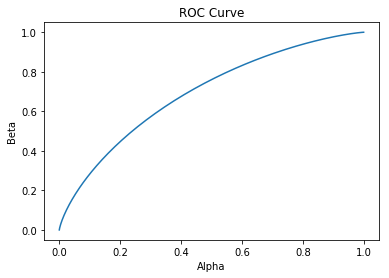
\includegraphics[scale=0.75]{ROCCurve.png}
\end{center}

\end{problemparts}

\newpage

\problem  % Problem 5

\begin{problemparts}

\problempart  % Problem 5a

Using Bayes' rule, the PPV can be written as,
$$ \mathbb{P}(H_1 \mid R) = \frac{\mathbb{P}(H_1) \cdot \mathbb{P}(R \mid
H_1)}{\mathbb{P}(R)} $$
Using the Law of Total Probability, this can be written in terms of known
quantities (assuming $H_0$ and $H_1$ span the universe),
\begin{align*}
    \mathbb{P}(H_1 \mid R) &= \frac{\mathbb{P}(H_1) \cdot \mathbb{P}(R \mid
    H_1)}{\mathbb{P}(H_0) \cdot \mathbb{P}(R \mid H_0) + \mathbb{P}(H_1)
    \cdot \mathbb{P}(R \mid H_1)} \\
    &= \boxed{\frac{\pi_1 \cdot \beta}{(1 - \pi_1) \cdot \alpha + \pi_1 \cdot
    \beta}}
\end{align*}
Substituting numerical values,
\begin{align*}
    \mathbb{P}(H_1 \mid R) &= \frac{0.0001 \cdot 0.99999}{(1 - 0.0001) \cdot
    0.05 + 0.0001 \cdot 0.99999} \\
    &\approx \boxed{0.00199619}
\end{align*}
Given the prior information that the alternative is expected to be very, very
rare, the significance level $\alpha$ needs to be much smaller to account for
this. If the $\alpha$ is reduced, the PPV will increase. An $\alpha =
0.000005$ will make the PPV approximately 95\%.

\problempart  % Problem 5b

Using Bayes' rule, the new PPV can be written as,
$$ \mathbb{P}(H_1 \mid R_m) = \frac{\mathbb{P}(H_1) \cdot \mathbb{P}(R_m \mid
H_1)}{\mathbb{P}(R_m)} $$
Using the Law of Total Probability (assuming $H_0$ and $H_1$ span the
universe), this becomes,
$$ \mathbb{P}(H_1 \mid R_m) = \frac{\mathbb{P}(H_1) \cdot \mathbb{P}(R_m \mid
H_1)}{\mathbb{P}(H_0) \cdot \mathbb{P}(R_m \mid H_0) + \mathbb{P}(H_1) \cdot
\mathbb{P}(R_m \mid H_1)} $$
Replacing $R_m$ with the provided expression,
$$ R_m = \bigcup_{i = 1}^n \left\{X_i \in R\right\} $$
Then the PPV becomes,
$$ \mathbb{P}(H_1 \mid R_m) = \frac{\mathbb{P}(H_1) \cdot
\mathbb{P}(\bigcup_{i = 1}^m \left\{X_i \in R\right\} \mid
H_1)}{\mathbb{P}(H_0) \cdot \mathbb{P}(\bigcup_{i = 1}^m \left\{X_i \in
R\right\} \mid H_0) + \mathbb{P}(H_1) \cdot \mathbb{P}(\bigcup_{i = 1}^m
\left\{X_i \in R\right\} \mid H_1)} $$
Using DeMorgan's law, 
\begin{align*}
    \mathbb{P}\left(R_m \mid H_0\right) &= \mathbb{P}\left(\bigcup_{i = 1}^m
    \left\{X_i \in R\right\} \mid H_0\right) \\
    &= 1 - \mathbb{P}\left(\left(\bigcup_{i = 1}^m \left\{X_i \in
    R\right\}\right)^c \mid H_0\right) \\
    &= 1 - \mathbb{P}\left(\bigcap_{i = 1}^m \left\{X_i \in R\right\}^c \mid
    H_0\right)
\end{align*}
Given that each $X_i$ are independent and identically distributed, 
\begin{align*}
    \mathbb{P}\left(R_m \mid H_0\right) &= 1 - \prod_{i = 1}^m
    \mathbb{P}\left(\left\{X_i \in R\right\}^c \mid H_0\right) \\
    &= 1 - \prod_{i = 1}^m \left(1 - \mathbb{P}\left(\left\{X_i \in R\right\}
    \mid H_0\right)\right)
\end{align*}
Using the provided values, this reduces to
\begin{align*}
    \mathbb{P}\left(R_m \mid H_0\right) &= 1 - \prod_{i = 1}^m \left(1 -
    \alpha\right) \\
    &= 1 - (1 - \alpha)^m
\end{align*}
The same is true for $\mathbb{P}(R_m \mid H_1)$,
$$ \mathbb{P}(R_m \mid H_1) = 1 - (1 - \beta)^m $$
Using these expressions, the PPV becomes,
$$ \mathbb{P}(H_1 \mid R_m) = \boxed{\frac{\pi_1 \cdot \left(1 - (1 -
\beta)^m\right)}{(1 - \pi_1) \cdot \left(1 - (1 - \alpha)^m\right) + \pi_1
\cdot \left(1 - (1 - \beta)^m\right))}} $$

\problempart  % Problem 5c

Using the previous values and $m = 10$, evaluating the PPV yields,
\begin{align*}
    \mathbb{P}(H_1 \mid R_{10}) &= \frac{0.0001 \cdot (1 - (1 -
    0.99999)^{10})}{(1 - 0.0001) \cdot (1 - (1 - 0.05)^{10}) + 0.0001 \cdot
    (1 - (1 - 0.99999)^{10})} \\
    &\approx \boxed{0.000249176}
\end{align*}
Given the observed data, the odds of $H_1$ being true is approximately $2.5$
times greater than before.

\end{problemparts}

\newpage

\problem  % Problem 6

Consider the following hypothesis,
$$ H_0 : \beta_0 = \beta_1 $$
$$ H_1 : \beta_0 \neq \beta_1 $$
If we let $\theta = \beta_0 - \beta_1$, this is equivalent to,
$$ H_0 : \theta = 0 $$
$$ H_1 : \theta \neq 0 $$
We can estimate $\beta_0$ and $\beta_1$,
$$ \hat{\beta}_0 = \bar{Y} - \hat{\beta}_1 \bar{X} $$
$$ \hat{\beta}_1 = \frac{\sum_{i = 1}^n (X_i - \bar{X})(Y_i -
\bar{Y})}{\sum_{i = 1}^n (X_i - \bar{X})^2} $$
We can write out the Wald statistic,
$$ W = \frac{\hat{\beta}_0 -
\hat{\beta}_1}{\sqrt{\hat{\mathrm{var}}(\hat{\beta}_0 - \hat{\beta}_1)}} $$
The variance of the estimate is given by,
$$ \hat{\mathrm{var}}(\hat{\beta}_0 - \hat{\beta}_1) =
\hat{\mathrm{var}}(\hat{\beta}_0) + \hat{\mathrm{var}}(\hat{\beta}_1) - 2
\hat{\mathrm{cov}}(\hat{\beta}_0, \hat{\beta}_1) $$
From lecture, the following variances are known,
$$ \hat{\mathrm{var}}(\hat{\beta}_0) = \frac{\hat{\sigma}^2(s_X^2 +
\bar{X}^2)}{n s_X^2},\ \hat{\mathrm{var}}(\hat{\beta}_1) =
\frac{\hat{\sigma}^2}{n s_X^2},\ \hat{\mathrm{cov}}(\hat{\beta}_0,
\hat{\beta}_1) = - \frac{\hat{\sigma}^2 \bar{X}}{n s_X^2} $$
Using the following estimate for $\hat{\sigma}^2$,
$$ \hat{\sigma}^2 = \frac{1}{n - 2} \sum_{i = 1}^n (y_i - \hat{\beta}_0 -
\hat{\beta}_1 x_i)^2 $$
Therefore, the $W$-statistic becomes,
$$ W = \frac{\hat{\beta}_0 - \hat{\beta}_1}{\sqrt{\frac{\hat{\sigma}^2(s_X^2
+ \bar{X}^2)}{n s_X^2} + \frac{\hat{\sigma}^2}{n s_X^2} + \frac{2
\hat{\sigma}^2 \bar{X}}{n s_X^2}}} $$
The statistic will approach the standard normal distribution. A two-sided
normal test with $\alpha = 0.05$, would be,
$$ \boxed{\mathbb{P}\left(\left|\frac{\hat{\beta}_0 -
\hat{\beta}_1}{\sqrt{\frac{\hat{\sigma}^2(s_X^2 + \bar{X}^2)}{n s_X^2} +
\frac{\hat{\sigma}^2}{n s_X^2} + \frac{2 \hat{\sigma}^2 \bar{X}}{n
s_X^2}}}\right| \geq 1.96\right) = 0.05} $$

\end{problems}

\end{document}
